\subsection{FizzleFade}
While most screen transition are done with a black fade effect (by shifting the palette), there are two instances
when the screen transition via fizzling:
\begin{itemize}
	\item When dying
	\item When killing a boss
\end{itemize}


Dying:\\
  \begin{figure}[H] \centering 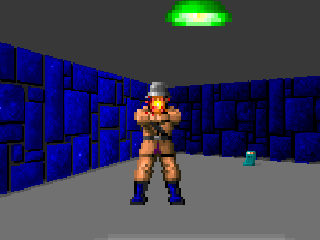
\includegraphics[scale=1.0]{imgs/fizzlefade/dying/screenshot_16.png} \end{figure}
    \begin{figure}[H] \centering 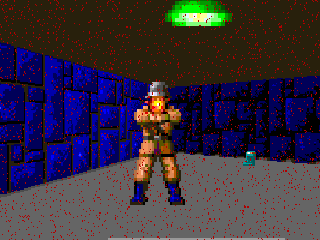
\includegraphics[scale=1.0]{imgs/fizzlefade/dying/screenshot_19.png} \end{figure}
      \begin{figure}[H] \centering 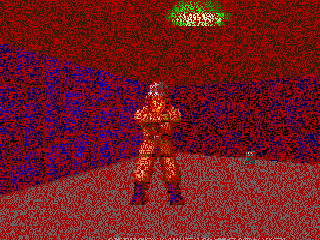
\includegraphics[scale=1.0]{imgs/fizzlefade/dying/screenshot_52.png} \end{figure}
        \begin{figure}[H] \centering 
\includegraphics[scale=1.0]{imgs/fizzlefade/dying/screenshot_86.png} \end{figure}

Boss:\\
\begin{figure}[H] \centering 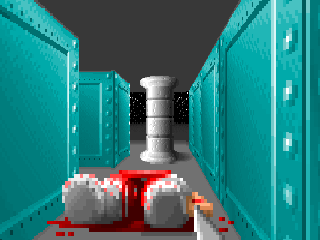
\includegraphics[scale=1.0]{imgs/fizzlefade/boss/screenshot_60.png} \end{figure}        
\begin{figure}[H] \centering 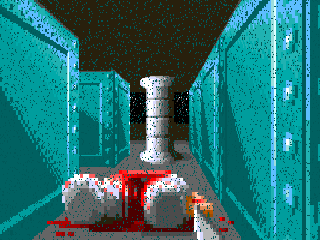
\includegraphics[scale=1.0]{imgs/fizzlefade/boss/screenshot_66.png} \end{figure}        
\begin{figure}[H] \centering 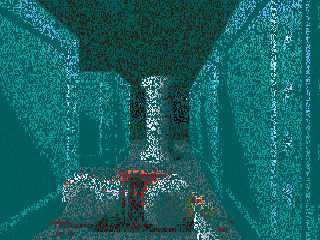
\includegraphics[scale=1.0]{imgs/fizzlefade/boss/screenshot_102.png} \end{figure}        
\begin{figure}[H] \centering 
\includegraphics[scale=1.0]{imgs/fizzlefade/boss/screenshot_130.png} \end{figure}        

The code responsible for this effect can be found in id\_vh.cpp, function FizzleFade. At first it is not obvious to understand how it works. I consider it to be one of the most beautiful trick of the engine:
\newpage
\lstinputlisting[language=C]{code/fizzlefade.c}

        \begin{figure}[H] \centering 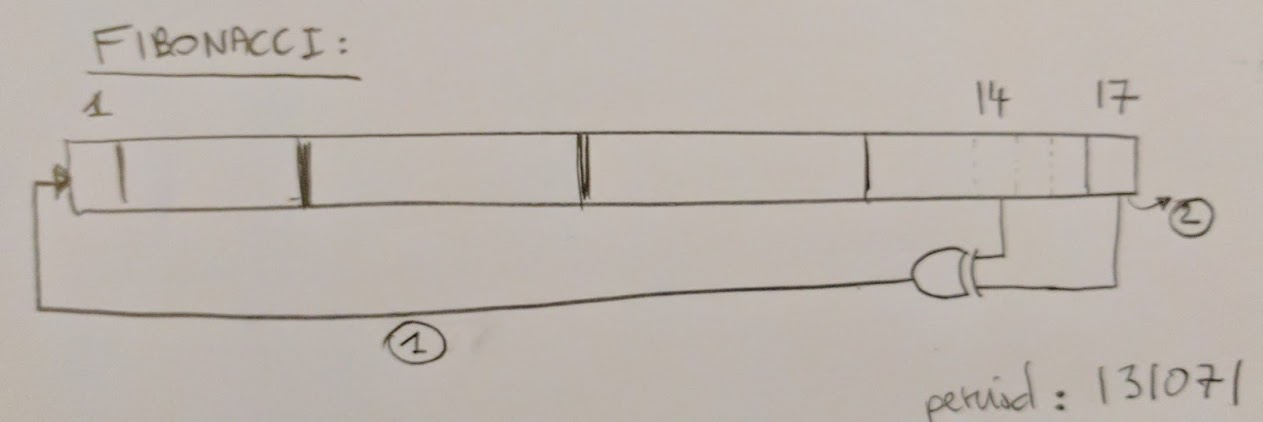
\includegraphics[scale=0.3]{imgs/fizzlefade/fibonnaci.png} \end{figure}
    \begin{figure}[H] \centering 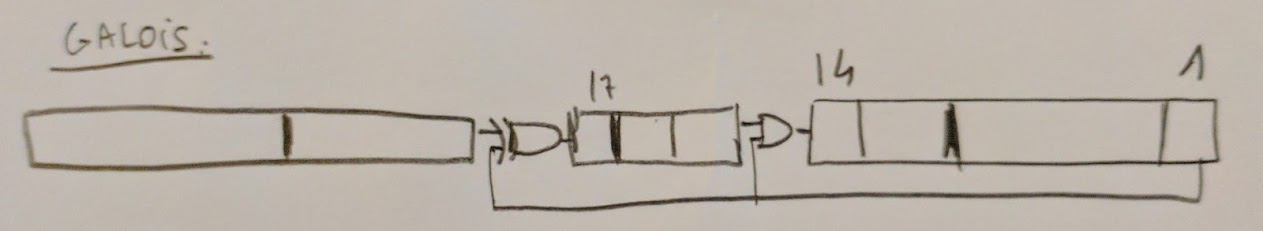
\includegraphics[scale=0.3]{imgs/fizzlefade/galois.png} \end{figure}
      
Note: Because the effect works by plotting pixels individually, this effect was very hard to replicate when developers tried to port the game to hardware accelerated GPU. As far as I know none of the port managed to replicate the fizzlefade.

Note: If you are curious about maximum-length taps, xilinx provides them from 3 to 168\footnote{Xilinx table can be found \href{http://www.xilinx.com/support/documentation/application\_notes/xapp052.pdf}{here}.}.